\chapter{Traffic danger ontology}
\label{cha:trafficDangerOntology}

\section{Introduction}
\label{sec:introductionTochapter3}

An ontology is described as formal representation of the knowledge about some domain, by a set of concepts within the domain, and the relationships between those concepts. It can be used either to define the domain, or to reason the properties of that domain. One of formal definitions of ontology is \textit{"formal, explicit specification of a shared conceptualization"} \cite{Gru93}. An ontology provides a shared vocabulary, which can be used to model a domain - that is, the type of objects and/or concepts that exist, and their properties and relations \cite{Arv08}.

Ontologies are used in artificial intelligence, Semantic Web, systems engineering, software engineering, biomedical informatics, etc. There are used as a form of knowledge representation about some part of world.

Ontologies may be represented by a lot of standards. Different ontology languages provide different facilities. The most recent development in standard ontology languages is OWL from the World Wide Web Consortium (W3C). One of the last tools for developing ontologies is Protégé \cite{OWLGuide}. Traffic danger ontology is developed using that tool. In Figure \ref{fig:annotations} there are annotations of that ontology, made in Protégé.

\medskip

\begin{figure}[htp]
\centering
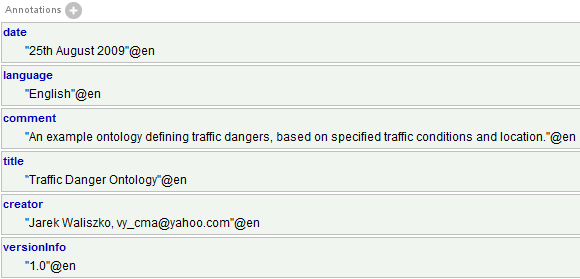
\includegraphics[scale=0.7]{images/chapter3/Annotations}
\caption{Traffic danger ontology annotations in Protégé}
\label{fig:annotations}
\end{figure}

\newpage

\begin{framed}
\noindent For the sake of clearness - almost all figures in this chapter refers to the traffic danger ontology and are all screenshots from Protégé tool. That assumption let avoid repeating under all figures the same supplement description (that figures are connected to traffic danger ontology, and are made in Protégé).
\end{framed}

\section{Knowledge engineering methodology for development of traffic danger concept}
\label{sec:knowledgeEngineering}

The real world provides a set of methodologies for developing an ontology, but there is no the fixed, best one. The domain experts can choose how to build ontologies in the way is best for them. While developing traffic danger ontology, the following fundamental rules described in \cite{OntDev101} were taken into consideration:
\begin{itemize}
    \item There is no one correct way to model a domain - there are always viable alternatives. The best solution almost always depends on the application that you have in mind and the extensions that you anticipate.
    \item Ontology development is necessarily an iterative process.
    \item Concepts in the ontology should be close to objects (physical or logical) and relationships in your domain of interest. These are most likely to be nouns (objects) or verbs (relationships) in sentences that describe your domain.
\end{itemize}

\noindent While developing an ontology it is important to have in mind that ontology is a model of real domain, so it must reflect reality. Details connected with that part of reality are going to be clearer and more crystallized down the road of building the ontology. After the initial version of the ontology, it is necessary to revise and rethink the design and repeat such iterative process to get the model that fulfill preferences and will be ready for giving answers for specific questions. Developing an ontology is not an aim on its own, usually it is a part of more complex software architecture which is driven by such formal domain model. Ontology should be applicable for the system it is going to cooperate. 

Methodology outlined above derives from agile development practices based on short feedback loops, systematic tests and constant cooperation with domain experts.

Ontology designing process requires to determine its domain and scope. It should be the starting point of work. That part is definitely more crystallized after answering several helpful questions \cite{OntDev101}:
\begin{itemize}
    \setlength{\itemsep}{0cm}
    \setlength{\parskip}{0cm}

    \item What is the domain that the ontology will cover?
    \item For what we are going to use the ontology?
    \item For what types of questions the information in the ontology should provide answers?
    \item Who will use and maintain the ontology?
\end{itemize}

\noindent The domain of traffic danger ontology consists of: traffic conditions, locations where such conditions can occur and the actual threats (related to specified conditions). The ontology will be used as the pillar of web system, which can provide real time information for traffic users about dangers connected with various areas. The ontology will be used by the public, it means, all end users who interact with the system. Besides, ontology will be widely accessible for anyone, who can use it for developing their own ideas based on that concept, or extend/improve existing formalization of the domain. Maintain of ontology will be narrowed for those trusted users, who can provide coherent, reliable data about current conditions on the roads. When it comes to competency questions \cite{FoxGru} the ontology is going to answer, traffic danger ontology passed through the following sample ones:
\begin{itemize}
    \setlength{\itemsep}{0cm}
    \setlength{\parskip}{0cm}

    \item What are the traffic dangers on specific area?
    \item Are there any dangers connected with low friction on specific area?
    \item What are the subareas of specific location?
    \item What kind of dangers are connected with bad atmospheric conditions?
    \item Is there any danger connected with specific postal code on specific district?
    \item Are there any traffic conditions provided for specific location?
\end{itemize}

\noindent After that part, domain developer should have almost clear vision of what knowledge structure is going to be created. Searching for already defined ontologies, which could fit desired problem, or at least some of its parts, is a good starting point. 

When it comes to the traffic danger ontology development process, the primary research has resulted in the finding of geographical locations ontology. Unfortunately that information structure was too complex to be included into the prototype. After all, it was not an easy task to find any helpful topics on the web - at least not formalized in a way simple enough that could be useful for the needs of this thesis. Because of that, creation of new ontology has started from scratch.

The top-down development process has been chosen for ontology creation. Starting from the definition of the most general concepts in the domain, ontology construction has been carried on, down to the most detailed concepts. After one concept had been entirely built up, and has been sufficient for the current needs, development of the next one has been started in the similar top-down way.

After all parts of ontology had been built, analysis of the ontology was started. The analysis procedure could be compared to specific kind of debugging process. In that part, reasoner was used for verifying answers for competency questions. If some parts of ontology was not coherent with another one, or the ontology was not able to result in providing correct answers, the broken parts were rebuilt. It was an iterative process, which ended when all competency questions was covered. Some of the questions has changed during the time of development process, but the latest form of the ontology fulfills answers to all questions correctly.

\section{Ontology parts description}
\label{sec:description}

In this section we will take a look at short outline of components that builds the OWL ontologies. We can talk about Individuals, Properties and Classes.

\subsection{Individuals}
\label{sub:individuals}

The individuals could be treated as instances of classes. They represent the concrete objects, in our domain. Figure \ref{fig:individuals} shows sample individuals, used in ontology we are talking about. 

\begin{framed}
\noindent These sample individuals shown below, are not present in the pure ontology which describes the prototype concept of traffic danger. Individuals, and all links connected to them, are added to ontology after synchronization with database, which I'll explain in Chapter \ref{cha:trafficDangerWebSystem}.
\end{framed}

\smallskip

\begin{figure}[htp]
\centering
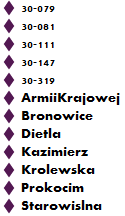
\includegraphics[scale=0.7]{images/chapter3/Individuals}
\caption{Sample individuals}
\label{fig:individuals}
\end{figure}

\newpage

\subsection{Properties}
\label{sub:properties}

Properties are binary relations between classes (or individuals). They account for linking individuals. In Figures \ref{fig:dataProperties} and \ref{fig:objectProperties} we can see respectively data and object properties used in traffic danger ontology.

\bigskip

\begin{figure}[htp]
\centering
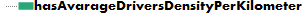
\includegraphics[scale=0.7]{images/chapter3/DataProperties}
\caption{Only one data property in our ontology}
\label{fig:dataProperties}
\end{figure}

\begin{figure}[htp]
\centering
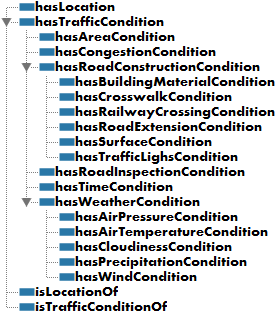
\includegraphics[scale=0.7]{images/chapter3/ObjectProperties}
\caption{Object properties}
\label{fig:objectProperties}
\end{figure}

\noindent Properties can have many features, e.g. they can have inverse properties, as discussed in the example below.

\bigskip

\noindent The property named \textbf{hasLocation} link the postal code individual \textbf{30-147} to the street individual called \textbf{ArmiiKrajowej} (Figure \ref{fig:armiiKrajowej}). The inverse property of \textbf{hasLocation} is \textbf{isLocationOf}. Because of the inversion, we can see, that the reasoner properly infer, that property \textbf{isLocationOf} link \textbf{ArmiiKrajowej} street to \textbf{30-147} postal code (Figure \ref{fig:30-147}). Inferred features are marked by light yellow background. The reasoning is based on description logics (DL), which will be explained later.

\medskip

\begin{figure}[htp]
\centering
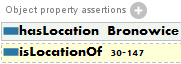
\includegraphics[scale=0.7]{images/chapter3/ArmiiKrajowej}
\caption{Property assertions (for the street named \textbf{ArmiiKrajowej} individual)}
\label{fig:armiiKrajowej}
\end{figure}

\begin{figure}[htp]
\centering
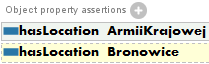
\includegraphics[scale=0.7]{images/chapter3/30-147}
\caption{Property assertions (for the postal code \textbf{30-147} individual)}
\label{fig:30-147}
\end{figure}

\newpage

\subsection{Classes}
\label{sub:classes}

If we use analogy, the classes may be viewed as types in object oriented programming. They represent the concepts, in the other words, they define the abstracts. They also may be treated as sets of individuals, and contain all individuals in our domain of concept, that fill all requirements of membership. Classes are though described using formal, mathematical descriptions called description logics (OWL DL). These logics allow, to precisely certify, if certain subclasses or individuals are members of our superclass, or not. The process of deduction may be computed automatically using reasoners. That is one of the key features of OWL-DL. Figure \ref{fig:individualsByClass} shows sample individuals assigned to their classes. Figure \ref{fig:assertedClassHierarchy} shows all classes, traffic danger ontology is consisted of.

\medskip

\begin{figure}[htp]
\centering
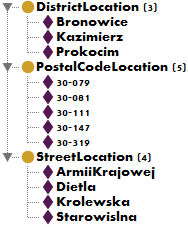
\includegraphics[scale=0.7]{images/chapter3/IndividualsByClass}
\caption{Individuals by class}
\label{fig:individualsByClass}
\end{figure}

\begin{figure}[htp]
\centering
\begin{tabular}[t]{ll}
\multirow{2}{*}{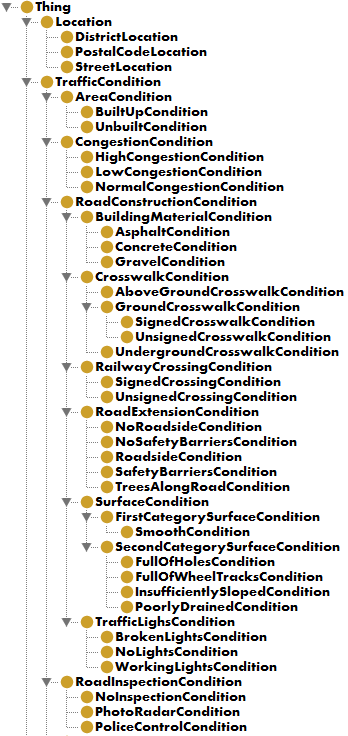
\includegraphics[scale=0.7]{images/chapter3/OntologyPart1}} & continuation... \vspace{0.6cm} \\
& 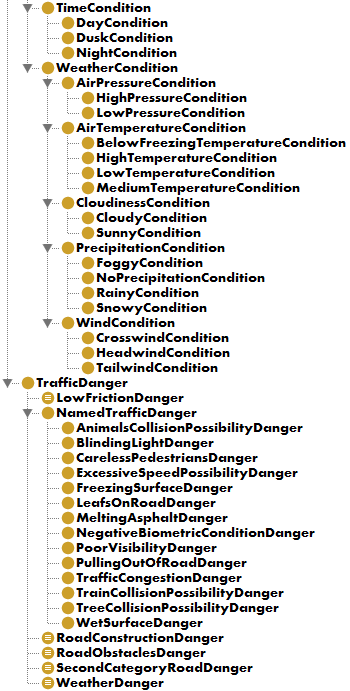
\includegraphics[scale=0.7]{images/chapter3/OntologyPart2}
\end{tabular}
\caption{Asserted class hierarchy}
\label{fig:assertedClassHierarchy}
\end{figure}

\newpage

\section{Existential and universal restrictions}
\label{sec:existentialAndUniversalRestrictions}

This section considers the important issue of existential and universal restrictions in Protégé. As it was described in Sections \ref{sec:dl} and \ref{sec:owl}, existential restrictions are denoted in formal Description Logics (DL) Syntax by $\mathit{existential~ quantifier} (\exists)$, and in Ontology Web Language (OWL) by $\mathit{someValuesFrom}$. Universal restrictions on the other hand, are denoted in DL Syntax by $\mathit{universal~ quantifier} (\forall)$, and in OWL by $\mathit{allValuesFrom}$.
\begin{itemize}
    \item \textit{"Existential restrictions describe classes of individuals that participate in at least one relationship along a specified property to individuals that are members of a specified class"} \cite{OWLGuide}. 

In Protégé the keyword \textbf{some} is used to denote existential restrictions.
    \item \textit{"Universal restrictions describe classes of individuals that for a given property only have relationships along this property to individuals that are members of a specified class"} \cite{OWLGuide}.

In Protégé the keyword \textbf{only} is used  to denote universal restrictions.
\end{itemize}

\section{Open world assumption and closure axiom}
\label{sec:openWorldAssumptionAndClosureAxiom}

This section is directly connected with the reasoning domain (see Section \ref{sec:reasoning}). The reason of separation this field to its individual section is to emphasize its importance.

Open word assumption (OWA) is one of the foundations of reasoning mechanisms used in Description Logics and OWL. In other papers OWA can be referred as OWR which extends to open world reasoning.

The OWA denotes, that a fact which has not been stated to be true, cannot be assumed to be false. In the other words there is prohibited to assume that something does not exist until that fact is explicitly stated. Such an ambiguous situation simply means that the knowledge has not yet been added to the knowledge base.

In the case of described traffic ontology, that is stated that \textbf{PoorVisibilityDanger} has precipitation conditions that are kinds of \textbf{FoggyCondition}, \textbf{RainyCondition} and \textbf{SnowyCondition}. Because of the open world assumption, until we explicitly say that a \textbf{PoorVisibilityDanger} only has that kinds of conditions, it is assumed (by the reasoner) that a \textbf{PoorVisibilityDanger} could have other conditions such as \textbf{SunnyCondition}. To specify explicitly that a \textbf{BlindingLightDanger} has conditions that are kinds of \textbf{FoggyCondition}, \textbf{RainyCondition} and \textbf{SnowyCondition} only, a closure axiom has to be added on the \textbf{hasPrecipitationCondition} property.

A closure axiom on a property denotes that property can be filled by the specified set of fillers. The axiom consists of a universal restriction which has a filler that is the union of fillers that occur in the existential restrictions for the property.

\newpage

In traffic danger ontology for example, the closure axiom on the \textbf{hasPrecipitationCondition} for \textbf{PoorVisibilityDanger} defined by following existential restrictions:

\[
\begin{array}{l} 
\exists hasPrecipitationCondition. FoggyCondition \\ 
\exists hasPrecipitationCondition. RainyCondition \\
\exists hasPrecipitationCondition. SnowyCondition
\end{array}
\]

\smallskip

{\tt \small
\begin{verbatim}
<owl:Class rdf:about="#PoorVisibilityDanger">
   <rdfs:label xml:lang="en">PoorVisibilityDanger</rdfs:label>
   <rdfs:subClassOf>
      <owl:Restriction>
         <owl:onProperty rdf:resource="#hasPrecipitationCondition"/>
         <owl:someValuesFrom rdf:resource="#FoggyCondition"/>
      </owl:Restriction>
   </rdfs:subClassOf>
   <rdfs:subClassOf>
      <owl:Restriction>
         <owl:onProperty rdf:resource="#hasPrecipitationCondition"/>
         <owl:someValuesFrom rdf:resource="#RainyCondition"/>
      </owl:Restriction>
   </rdfs:subClassOf>
   <rdfs:subClassOf>
      <owl:Restriction>
         <owl:onProperty rdf:resource="#hasPrecipitationCondition"/>
         <owl:someValuesFrom rdf:resource="#SnowyCondition"/>
      </owl:Restriction>
   </rdfs:subClassOf>
</owl:Class>
\end{verbatim}
}

\medskip

\begin{figure}[htp]
\centering
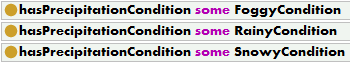
\includegraphics[scale=0.7]{images/chapter3/ClosureAxiomPart1}
\caption{Existential restrictions on \textbf{hasPrecipitationCondition} property}
\label{fig:existentialRestrictions}
\end{figure}

\newpage

\noindent is stated as a universal restriction, which acts along the \textbf{hasPrecipitationCondition} property, with a filler that is the union of \textbf{FoggyCondition}, \textbf{RainyCondition} and also \textbf{SnowyCondition}:

\[
\forall hasPrecipitationCondition. (FoggyCondition \sqcup RainyCondition \sqcup SnowyCondition)
\]

\smallskip

{\tt \small
\begin{verbatim}
<owl:Class rdf:about="#PoorVisibilityDanger">
   <rdfs:subClassOf>
      <owl:Restriction>
         <owl:onProperty rdf:resource="#hasPrecipitationCondition"/>
         <owl:allValuesFrom>
            <owl:Class>
               <owl:unionOf rdf:parseType="Collection">
                  <rdf:Description rdf:about="#FoggyCondition"/>
                  <rdf:Description rdf:about="#RainyCondition"/>
                  <rdf:Description rdf:about="#SnowyCondition"/>
               </owl:unionOf>
            </owl:Class>
         </owl:allValuesFrom>
      </owl:Restriction>
   </rdfs:subClassOf>
</owl:Class>
\end{verbatim}
}

\medskip

\begin{figure}[htp]
\centering
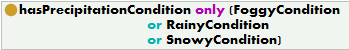
\includegraphics[scale=0.7]{images/chapter3/ClosureAxiomPart2}
\caption{Closure axiom on \textbf{hasPrecipitationCondition} property}
\label{fig:closureAxiom}
\end{figure}

\newpage

\section{Reasoning}
\label{sec:reasoning}

\subsection{Introduction}
\label{sub:introduction}

Such classes that do not have any sets of necessary and sufficient conditions, but have only necessary conditions, are known as primitive classes. In Protégé they are marked by plain round yellow icon. Yet the classes marked by 3 horizontal white lines, are called defined classes. It means that such classes have at least one set of the necessary and sufficient conditions for the reasoner, to make assumptions based on their descriptions (to infer relationships). The reasoner is able to infer dependencies only for defined classes \cite{OWLGuide}. When we turn on the reasoner, the result of inferred classes will be like that presented in Figure \ref{fig:inferredClassHierarchy}.

\medskip

\begin{figure}[htp]
\centering
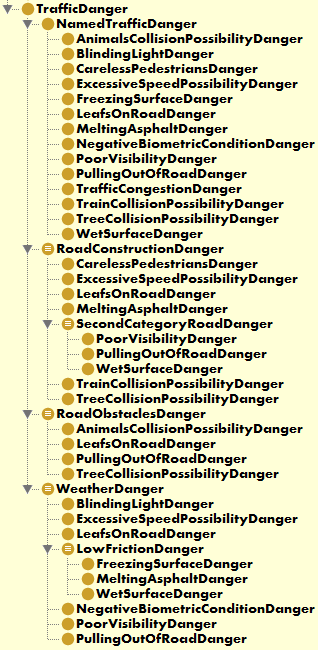
\includegraphics[scale=0.67]{images/chapter3/InferredClassHierarchy}
\caption{Defined classes with inferred memberships from \textbf{NamedTrafficDanger} subclasses}
\label{fig:inferredClassHierarchy}
\end{figure}

\newpage

\noindent Another view of this taxonomy can be generated using Graphviz tool. It is open source graph (network) visualization project from AT\&T Research. Graphviz is integrated with Protégé as a plugin called OWLViz. We can take a look of \textbf{TrafficDanger} class subclasses structure in Figure \ref{fig:trafficDangerOwlViz}.

\medskip

\begin{figure}[htp]
\centering
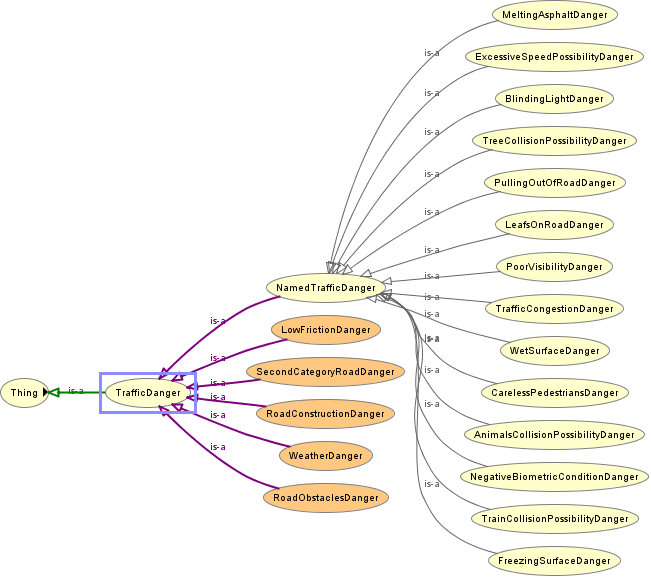
\includegraphics[scale=0.7]{images/chapter3/TrafficDangerOwlViz}
\caption{Graphviz made view showing subclasses structure of \textbf{TrafficDanger} class}
\label{fig:trafficDangerOwlViz}
\end{figure}

\noindent That orange ellipses shows the defined classes, which we were talking about earlier. The light yellow ellipses show primitive types. At the above picture we can see all subclasses of \textbf{NamedTrafficDanger} class. All of them have conditions based on which reasoner can make assumptions, and infer them to according defined classes. After inferring we can use OWLViz to show us the inferred relationships. Figure \ref{fig:weatherDangerInferredOwlViz} shows the inferred memberships of \textbf{WeatherDanger} class.

\newpage

\begin{figure}[htp]
\centering
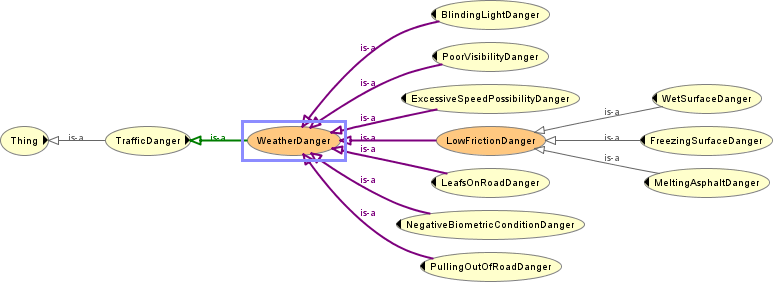
\includegraphics[scale=0.6]{images/chapter3/WeatherDangerInferredOwlViz}
\caption{Inferred members of \textbf{WeatherDanger} type}
\label{fig:weatherDangerInferredOwlViz}
\end{figure}

\noindent The reasoner infer memberships of \textbf{WeatherDanger} type. We can see that \textbf{LowFrictionDanger} defined class is also subclass of \textbf{WeatherDanger}. Additionally that class has its own deducted members such as: \textbf{WetSurfaceDanger}, \textbf{FreezingSurfaceDanger} and \textbf{MeltingAsphaltDanger}.

How the classes were inferred, to be finally matched under appropriate supertypes? It is all because of description logics, the reasoning process of the reasoner engine is based on.

\subsection{First example}
\label{sub:firstExample}

In this example \textbf{LowFrictionDanger} deduction case is exercised. Below, in Figure \ref{fig:lowFrictionDanger}, we can see DL description, which tell us something about that class.

\medskip

\begin{figure}[htp]
\centering
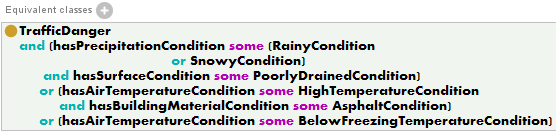
\includegraphics[scale=0.7]{images/chapter3/LowFrictionDanger}
\caption{OWL DL description of \textbf{LowFrictionDanger}}
\label{fig:lowFrictionDanger}
\end{figure}

\noindent Based on DL description, the subclasses tree is build. All we want to do is to classify specific dangers from \textbf{NamedTrafficDanger} type, to wider danger type called \textbf{LowFrictionDanger}. For that danger to occur, the following complex criteria must be fulfilled:

\newpage
\begin{enumerate}
    \setlength{\itemsep}{0cm}
    \setlength{\parskip}{0cm}

    \item there has to occur precipitation like rain or snow, and simultaneously the road has to have damaged system of draining water out from surface, or
    \item the air temperature has to be high while we are driving on asphalt road, or finally
    \item the temperature has to be below freezing, (because the surface is frozen and hence slippery)
\end{enumerate}

\noindent Because we know now (from Figure \ref{fig:weatherDangerInferredOwlViz}), the inferred members of \textbf{LowFrictionDanger} (\textbf{WetSurfaceDanger}, \textbf{FreezingSurfaceDanger} and \textbf{MeltingAsphaltDanger}), we should take a look of theirs DL descriptions. Figures \ref{fig:wetSurfaceDanger}, \ref{fig:freezingSurfaceDanger} and \ref{fig:meltingAsphaltDanger} show the dangers in mentioned order.

\medskip

\begin{figure}[htp]
\centering
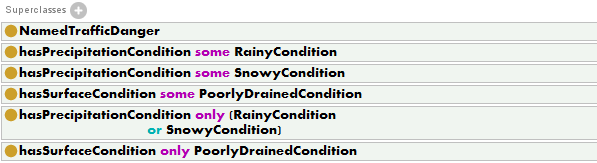
\includegraphics[scale=0.7]{images/chapter3/WetSurfaceDanger}
\caption{\textbf{WetSurfaceDanger} concept superclasses set}
\label{fig:wetSurfaceDanger}
\end{figure}

\begin{figure}[htp]
\centering
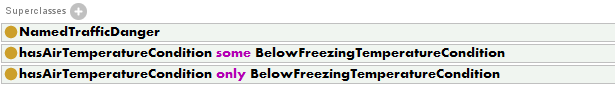
\includegraphics[scale=0.7]{images/chapter3/FreezingSurfaceDanger}
\caption{\textbf{FreezingSurfaceDanger} concept superclasses set}
\label{fig:freezingSurfaceDanger}
\end{figure}

\begin{figure}[htp]
\centering
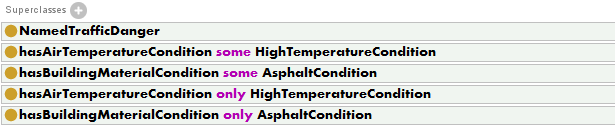
\includegraphics[scale=0.7]{images/chapter3/MeltingAsphaltDanger}
\caption{\textbf{MeltingSurfaceAsphalt} concept superclasses set}
\label{fig:meltingAsphaltDanger}
\end{figure}

\newpage

\noindent If we spent a while on analyzing the descriptions, the deduction which reasoner makes should by obvious and easy. Take a closer look at \textbf{FreezingSurfaceDanger} (Figure \ref{fig:freezingSurfaceDanger}). We can see that such a cold situation may occur only when the temperature is lower than 0. That is necessary condition that has to occur for the class, to be matched. \textbf{BelowFreezingTemperatureCondition} is defined as a subset of \textbf{AirTemperatureCondition}, and that one in turn is a subset of \textbf{WeatherCondition} (Figure \ref{fig:belowFreezingTemperatureConditionOWLViz}).

\medskip

\begin{figure}[htp]
\centering
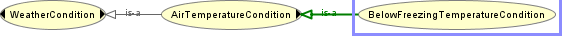
\includegraphics[scale=0.7]{images/chapter3/BelowFreezingTemperatureConditionOWLViz}
\caption{Superclasses path of \textbf{BelowFreezingTemperatureCondition} class}
\label{fig:belowFreezingTemperatureConditionOWLViz}
\end{figure}

\noindent The description of \textbf{WeatherDanger} class (Figure \ref{fig:weatherDanger}) tells, that such kinds of dangers can be caused by inappropriate weather conditions.

\medskip

\begin{figure}[htp]
\centering
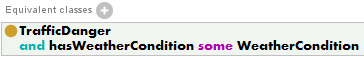
\includegraphics[scale=0.7]{images/chapter3/WeatherDanger}
\caption{\textbf{WeatherDanger} concept superclasses set}
\label{fig:weatherDanger}
\end{figure}

\noindent Because \textbf{BelowFreezingTemperatureCondition} is weather condition (subset of \textbf{WeatherCondition} type), \textbf{FreezingSurfaceDanger} is a member of \textbf{WeatherDanger} type.

\subsection{Second example}
\label{sub:secondExample}

We can take a closer look at another example of reasoning. This time we will ask the ontology to fetch dangers, which may occur on district named \textbf{StareMiasto}. There is no class prepared for answering such a question on class hierarchy shown in Figure \ref{fig:assertedClassHierarchy}. We have to write the query directly, using DL Query tab in Protégé. Below, in Figure \ref{fig:query}, the complete query is prepared. 

\medskip

\begin{figure}[htp]
\centering
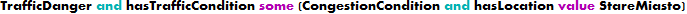
\includegraphics[scale=0.7]{images/chapter3/Query}
\caption{Query for dangers possibilities on district \textbf{StareMiasto}}
\label{fig:query}
\end{figure}

\noindent More precisely, the query fetches all classes of dangers, raised as a results of road conditions appeared on district \textbf{StareMiasto}.

We have to inform ontology about some details, for associated reasoner to give the correct answer. I would like to show how it can be done using Protégé editor. It is why I have prepared simple tutorial. In the next few steps we will add required information. The information we are going to add is appropriate just for this example, and can be very different in reality.

\begin{framed}
\noindent The analogical process, of filling ontology with additional knowledge, is called \textit{synchronization} in this paper. It is done automatically, as a part of functionality provided by a system described in the Chapter \ref{cha:trafficDangerWebSystem}. The detailed information will be provided later.
\end{framed}

\noindent We are going to execute following steps using Protégé:

\begin{enumerate}
    \setlength{\itemsep}{0cm}
    \setlength{\parskip}{0cm}

    \item Create individuals: postal code \textbf{30-020}, street \textbf{Szpitalna}, and district \textbf{StareMiasto}. The postal code should belong to street, and the street should belong to district (through \textbf{hasLocation} relation). Filling ontology with new individuals data is done using Protégé \textit{Individuals} tab:
    \begin{itemize}
        \setlength{\itemsep}{0cm}
        \setlength{\parskip}{0cm}

        \item add \textbf{hasLocation} relation to appropriate individual, by repeating following process for postal code and street:
        \begin{itemize}
            \setlength{\itemsep}{0cm}
            \setlength{\parskip}{0cm}

            \item select appropriate individual on \textit{Individuals} tree,
            \item click on \textit{Object property assertions} button in the \textit{Property assertions} window,
            \item in the opened window write \textit{"hasLocation Szpitalna"} for postal code \textbf{30-020} and \textit{"hasLocation StareMiasto"} for \textbf{Szpitalna} street,
        \end{itemize}

        \item define types for provided individuals, by repeating following process for postal code, street and district:
        \begin{itemize}
            \setlength{\itemsep}{0cm}
            \setlength{\parskip}{0cm}

            \item select appropriate individual on \textit{Individuals} tree,
            \item click on \textit{Types} button on \textit{Description} tab,
            \item in the opened window write appropriate type for each individual: \textit{"PostalCodeLocation"} for \textbf{30-020}, \textit{"StreetLocation"} for \textbf{Szpitalna}, and \textit{"DistrictLocation"} for \textbf{StareMiasto}.
        \end{itemize}

    \end{itemize}

    \item Associate the location defined by postal code \textbf{30-020} with \textbf{HighCongestionCondition} condition, to assert that such a condition occurs in this area. That process is done using \textit{Classes} tab:
    \begin{itemize}
        \setlength{\itemsep}{0cm}
        \setlength{\parskip}{0cm}

        \item select \textit{HighCongestionCondition} node on \textit{Asserted class hierarchy} tree,
        \item click \textit{Superclasses} button,
        \item write \textit{"hasLocation value 30-020"} in the newly opened window.
    \end{itemize}

\end{enumerate}

\noindent Now ontology is prepared. We can execute query shown in Figure \ref{fig:query} using DL Query tab. After executing, there will be one subclass in the result set. It is \textbf{TrafficCongestionDanger}. Take a closer look on description of that class, in order to understand why it has been fetched. In Figure \ref{fig:trafficCongestionDanger} we can see, that \textbf{TrafficCongestionDanger} class is connected to \textbf{HighCongestionDanger} condition.

\newpage

\begin{figure}[htp]
\centering
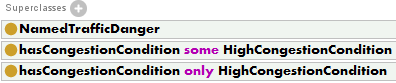
\includegraphics[scale=0.7]{images/chapter3/TrafficCongestionDanger}
\caption{\textbf{TrafficCongestionDanger} concept superclasses set}
\label{fig:trafficCongestionDanger}
\end{figure}

\noindent Taking under consideration connections between postal code, street, and district individuals (Figure \ref{fig:connection}), reasoner can assume, that postal code area \textbf{30-020} belongs to \textbf{StareMiasto} district. 

\medskip

\begin{figure}[htp]
\centering
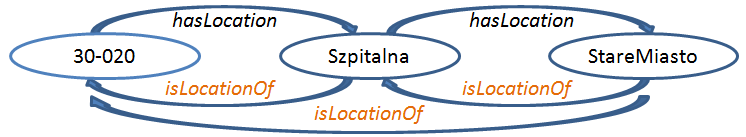
\includegraphics[scale=0.6]{images/chapter3/Connection}
\caption{Connections chain from postal code to district}
\label{fig:connection}
\end{figure}

\noindent The reasoner deduction for \textbf{StareMiasto} is shown in Figure \ref{fig:stareMiasto}.

\medskip

\begin{figure}[htp]
\centering
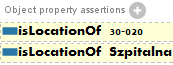
\includegraphics[scale=0.7]{images/chapter3/StareMiasto}
\caption{Inferred property assertions for \textbf{StareMiasto} district}
\label{fig:stareMiasto}
\end{figure}

\noindent In the above steps, we have synchronized the core ontology with sample knowledge. The way we have done that (information shown in Figure \ref{fig:trafficCongestionDanger} and Figure \ref{fig:stareMiasto}) allow to deduct, that \textbf{TrafficCongestionDanger} occurs on \textbf{StareMiasto} district.

\section{Summary}
\label{sub:ontologyDevelopementSummary}

Modern ontology development tools such as Protégé allow users to exploit ontologies conveniently, and provide intelligent guidance to find mistakes similar to a debugger in a programming environment. The only thing users have to do, for classes classification and inconsistencies detection process to be executed, is to choose a \textit{Classify} option shown in Figure \ref{fig:classify}.

\newpage

\begin{figure}[htp]
\centering
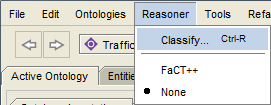
\includegraphics[scale=0.7]{images/chapter3/Classify}
\caption{Reasoner invoking in Protégé}
\label{fig:classify}
\end{figure}

\noindent In addition, Protégé is ideal as a rapid prototyping environment in which ontology designers can instantly create individuals of specific classes in their ontology and experiment with semantic restrictions \cite{OntDrivDev}.

Furthermore, as a support for ontology researchers, Protégé has an open architecture and is easily extensible. That allows programmers to integrate arbitrary components with the tool. As a result ontology designers have a wide range of third-party plugins, which they can use. Protégé plugin library can be found under wiki page of the tool \cite{ProtegeWiki}. 
